\pagestyle{fancy}

This text is a companion to \textit{Introductory Statistics for the Life and Biomedical Sciences}; while the main text focuses on a conceputal introduction to the use of statistics in the life sciences, this supplement provides an analytical and computational introduction using the statistical computing language \textsf{R}.  An understanding of the basics of \textsf{R}, how it stores, utilizes, and processes data, and how to analyze these results will be built.  

\section{What is \textsf{R}?}
\textsf{R} is an open-source statistical software that allows users to import, transform, and analyze data in order to draw conclusions.  In this case, it will be used to perform analyses of biomedical data, and this text will go through the steps to do so from installation to drawing conclusions.  

\subsection{Installation of \textsf{R}}
\textsf{R} is freely available on the internet, and it is recommended to download it from \url{http://cran.us.r-project.org/}, where there are up to date versions for Windows, Mac OS X, and Linux.  This link will provide instructions for a complete download.  

\subsection{Introduction to RStudio}
\textsf{RStudio} is a platform that makes using \textsf{R} significantly easier, providing a visual framework for working. It can be downloaded from \url{https://www.rstudio.com/products/rstudio/download/}, by scrolling to the bottom and selecting the appropriate operating system from \textit{Installers} under \textit{Installers for Supported Platforms}.  \textsf{RStudio} is not necessary in order to use \textsf{R}, but it is highly recommended for organizational and accesibility reasons.      


Upon opening \textsf{RStudio}, something similar to Figure \ref{fig:rstudio} should appear.  The four pane window environment is standard and provides easy access to many of the most commonly utilized tools.  Note that the four panes can be moved around or closed, so different versions of \textsf{Rstudio} may look a bit different.  
\begin{figure}[h!]
\centering
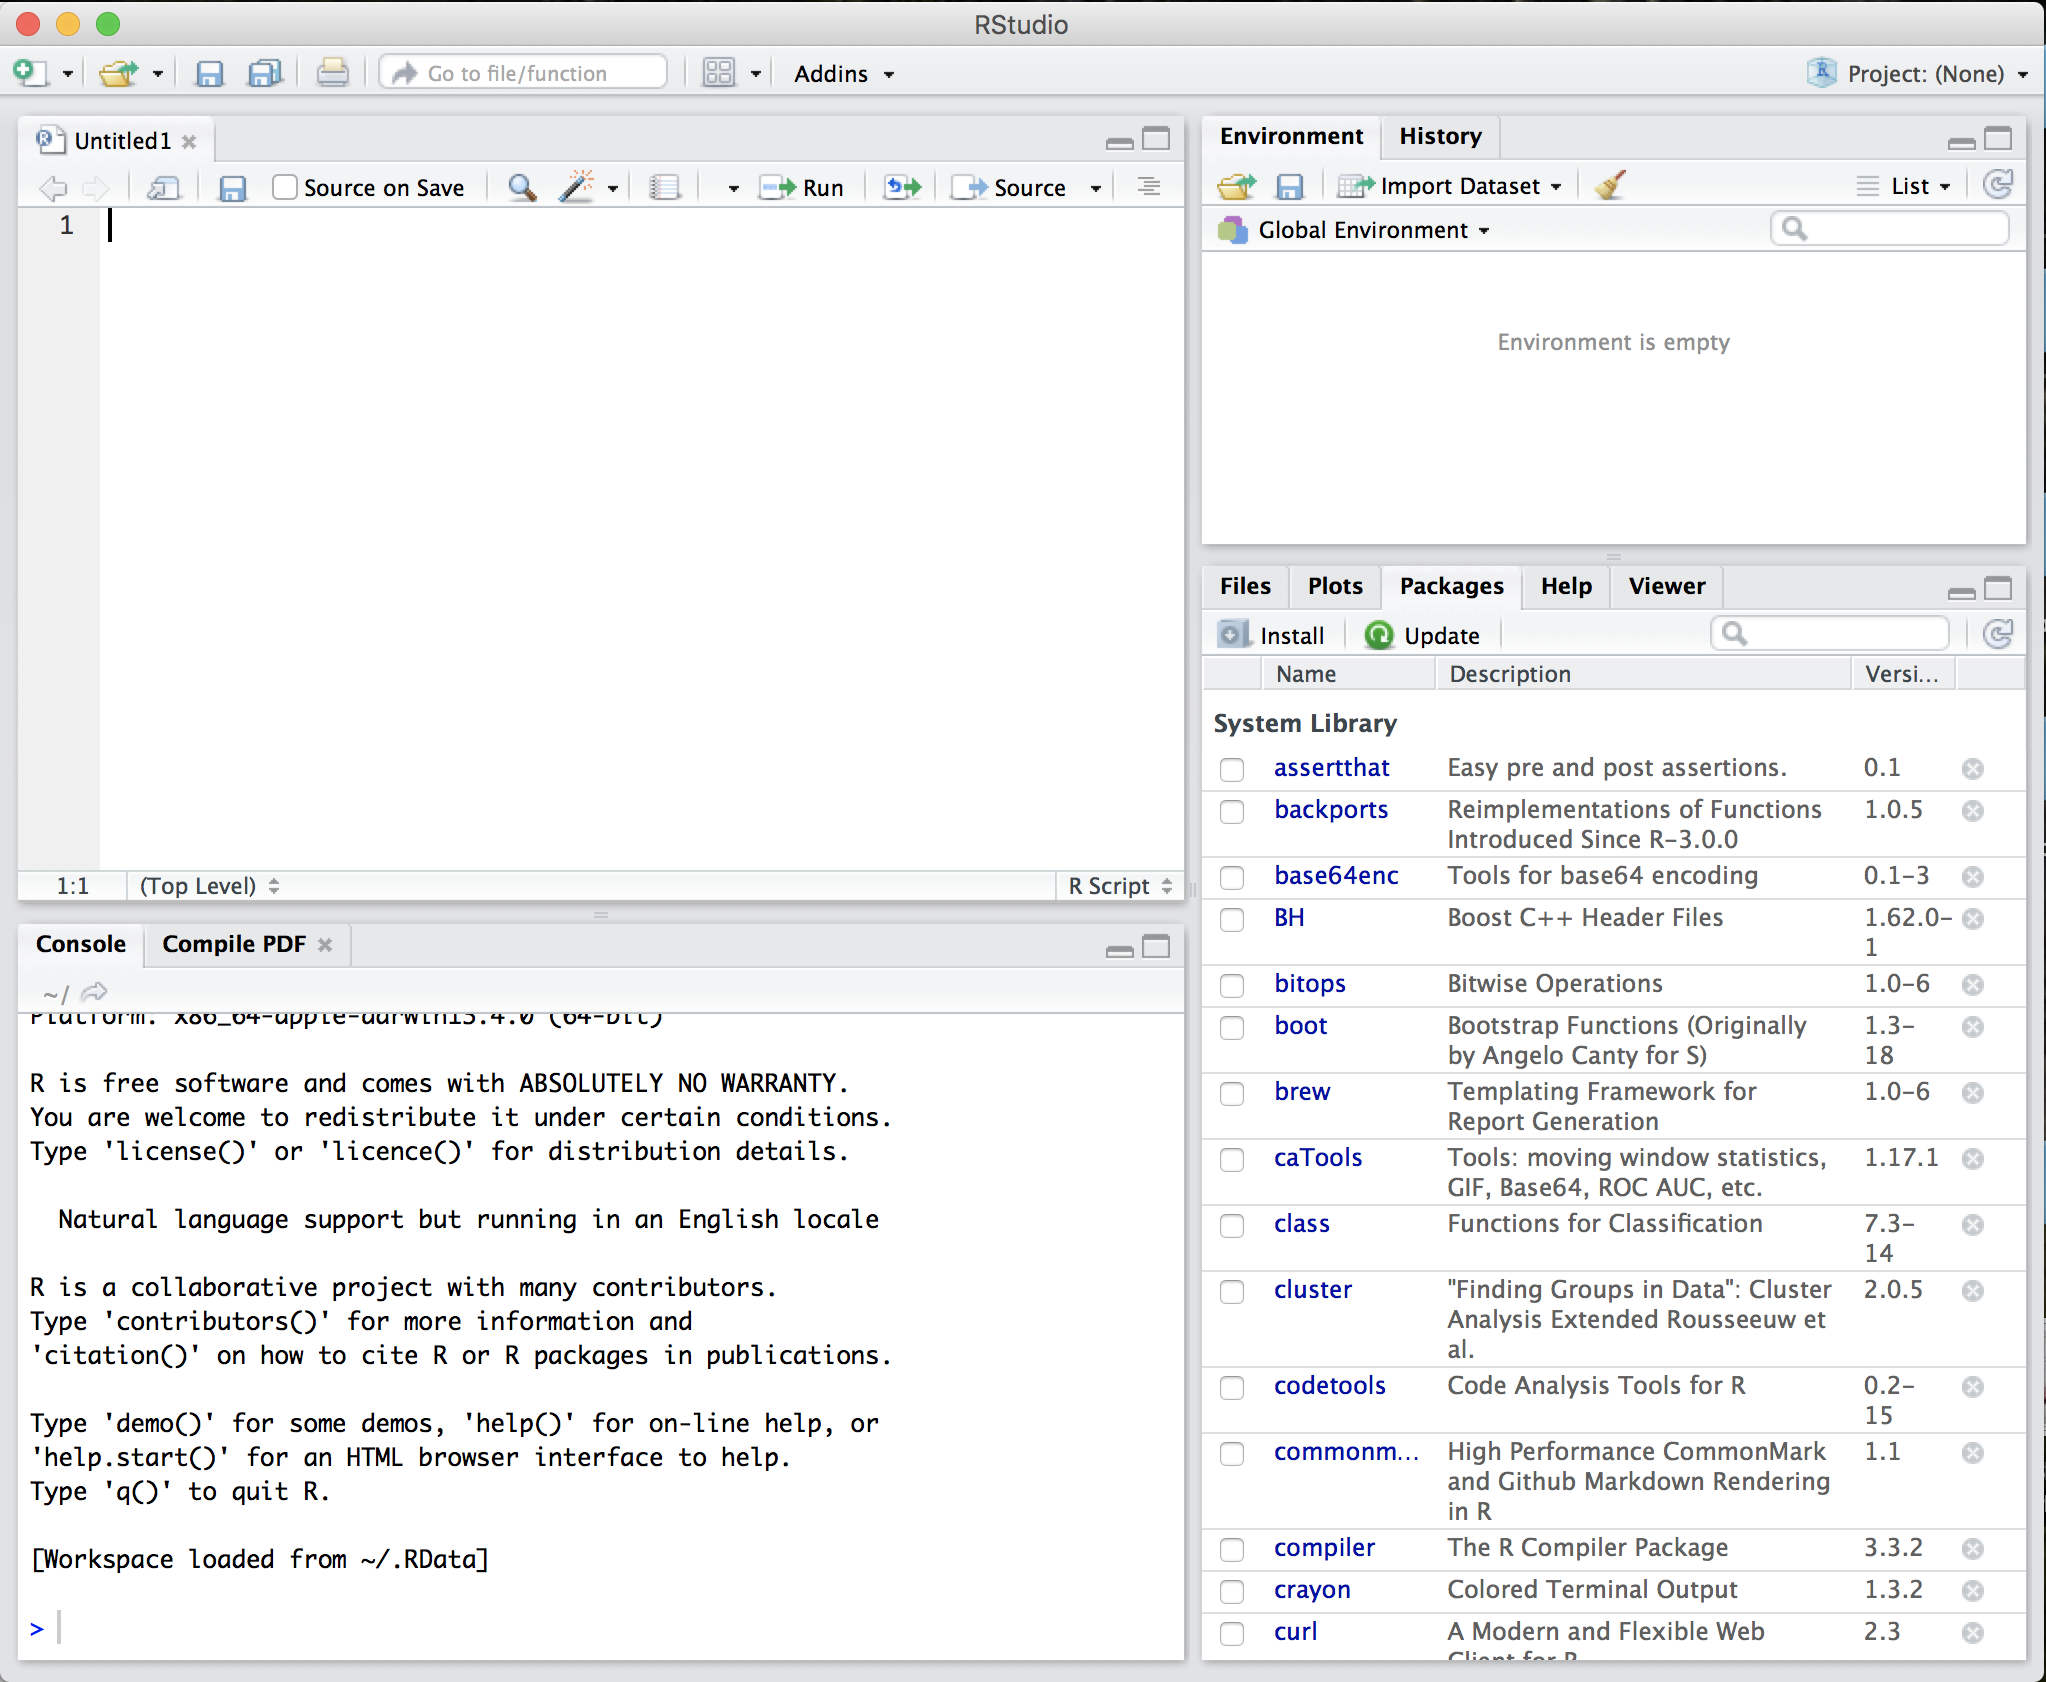
\includegraphics[width = 6in]{chapters/chapter_0/rstudio.png}
\caption{The default \textsf{RStudio} layout.  }
\label{fig:rstudio}
\end{figure}

\subsubsection{The Script Editor}
The top left pane in Figure \ref{fig:rstudio} shows the script editor, used to edit a \textsf{R} script file.  Think of this pane as similar to any text editor, providing a working space for the code being utilized and a means to save that for later.  We recommend that all work is done in a \textsf{R} script file so no information is lost.  If a script editor is not visible, a new \textsf{R} script file can be created by going to \textit{File > New File > R Script}.  

In order to run a command in the script editor, you must place your curser on the line you want to run and type \textsf{command + Return} on Mac or \textsf{Ctrl + Enter} on Windows or Linux.  Alternatively, at the top of the script editor pane is the run button, which can be clicked after highlighting the code to be run.  Try this for yourself with the following example, and if successful, you shall see "hi" print out in the bottom left pane.  

\begin{knitrout}
\definecolor{shadecolor}{rgb}{0.969, 0.969, 0.969}\color{fgcolor}\begin{kframe}
\begin{alltt}
\hlkwd{print}\hlstd{(}\hlstr{"hi!"}\hlstd{)}
\end{alltt}
\begin{verbatim}
## [1] "hi!"
\end{verbatim}
\end{kframe}
\end{knitrout}


\subsubsection{The Console} 
The bottom left pane in Figure \ref{fig:rstudio} is called the console.  This is the machinery in \textsf{R} that does the actual computing.  When commands are run in the script editor, they show up in the console, so the console is an important pane to always have in your \textsf{RStudio environment}.  

\subsubsection{The Environment Tab} 
The top right pane in Figure \ref{fig:rstudio} shows the \textsf{Environment} tab, which is the home of all stored information in \textsf{R}, such as datasets and variables.  The creation of any variables will show up here.  For example, upon running the following command in the script editor, a variable called \textit{x} should come up under \textsf{Values} in the \textsf{Environment} tab. The equals sign in the command below indicates that the variable of name \textsf{x} is taking on the numerical value 2. A variable created in this way is stored in \textsf{R} for later use and can later be called upon by referencing its variable name, \textit{x}.  Examples of this will be shown in Section \ref{}.  

\begin{knitrout}
\definecolor{shadecolor}{rgb}{0.969, 0.969, 0.969}\color{fgcolor}\begin{kframe}
\begin{alltt}
\hlstd{x} \hlkwb{=} \hlnum{2}
\end{alltt}
\end{kframe}
\end{knitrout}


Furthermore, this pane can be used to import a dataset, and if successful, you should see the dataset show up in this global environment.  A dataset can be imported using the button \textit{Import Dataset} or from the script editor using the command \textit{load()} with the dataset name in quotation marks inside the parentheses.  For example, using a dataset that is on the local machine, the following will import the dataset into \textsf{R} for use and will show up in the \textsf{Environment} pane under \textsf{Data}, 

%% Wherever we upload the book online, we may want to post this dataset and hyperlink it here so people can see the example.  I think this is an important point for people to know how to upload their own datasets.  

\begin{knitrout}
\definecolor{shadecolor}{rgb}{0.969, 0.969, 0.969}\color{fgcolor}\begin{kframe}
\begin{alltt}
\hlkwd{load}\hlstd{(}\hlstr{"samp_df.Rda"}\hlstd{)}
\end{alltt}
\end{kframe}
\end{knitrout}


At this point, the global environment looks something like that seen in Figure \ref{fig:rstudioenv}, showing both the variable \textit{x} and the dataset \textit{samp.df}.  
\begin{figure}[h!]
\centering
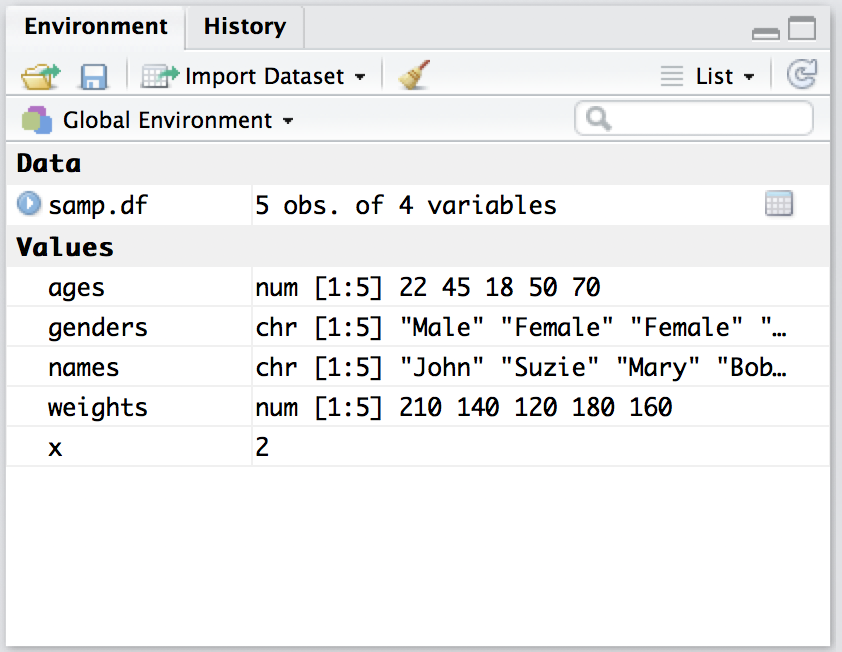
\includegraphics[width = 2in]{chapters/chapter_0/rstudioenv.png}
\caption{An example of how the global environment stores datasets and variables.}
\label{fig:rstudioenv}
\end{figure}


\subsubsection{The Files Tab}
In the lower right pane of Figure \ref{fig:rstudio}, several tabs can be seen.  The Files tab is a directory of all the files on the local computer and can be used to access other files, such as saved datasets or previously created \textsf{R} scripts.  

\subsubsection{The Plots Tab} 
The next tab seen is the Plots tab, which is where plots will be displayed when created in a R script file.  Section \ref{graphs} will go into more detail as to how to create plots, but just note that this is where they will show up.  

\subsubsection{The Packages Tab}
Because \textsf{R} is an open-source software, anyone can creates packages for it that contain functions, data, or other useful programs.  Packages are then shared and built upon to make the knowledge base of the community greater.  The Packages tab is where these packages are accessible in \textsf{RStudio}.  Many packages come standard with the installation of \textsf{RStudio} and can be seen here.  By checking the box to the left of a package, all of its contents will be available for use.  A package has been created to accompany this book, and it can be included for use in the packages tab.  Section \ref{thepackage} will discuss this specific package in further detail.  



\section{The OIBioStat Package} \label{thepackage}
All the datasets used in the text can be accessed by downloading the OIBiostat package from \textsf{R}. Run the following command to download the package:
%' 
%' %% These commands aren't going to work until we have uploaded the package to CRAN. Just skip it for now and require below.
% <<eval = FALSE>>=
% install.packages("OIBioStat")  ## make sure to include the quotations
% @
%' 


Each time the package is needed, run the following command: 
%' 
\begin{knitrout}
\definecolor{shadecolor}{rgb}{0.969, 0.969, 0.969}\color{fgcolor}\begin{kframe}
\begin{alltt}
\hlkwd{require}\hlstd{(OIBioStat)}
\end{alltt}
\end{kframe}
\end{knitrout}

To access a dataset in the package, simply run the \texttt{data()} command, which will load it into the \textsf{R} environment.  To see this has been done, it will pop up in the top right of \textsf{RStudio} in the pane labeled \textit{Environment} under \textit{Data}.  For example, a dataset called \texttt{swim} is in the package and can be loaded as follows, 
\begin{knitrout}
\definecolor{shadecolor}{rgb}{0.969, 0.969, 0.969}\color{fgcolor}\begin{kframe}
\begin{alltt}
\hlkwd{data}\hlstd{(swim)}
\end{alltt}
\end{kframe}
\end{knitrout}

